\begin{frame}{Regression Example}
    Asking \texttt{R} for a summary of the regression model, we get the following:
    \begin{center}
        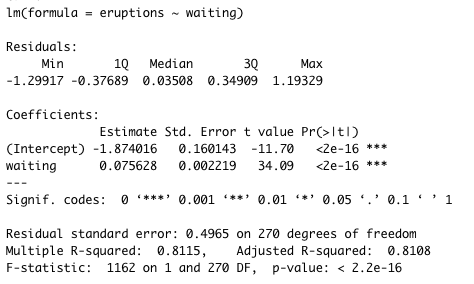
\includegraphics[scale=0.6]{images/regsum.png}
    \end{center}
    Let's pick this apart piece by piece.
\end{frame}

\begin{frame}{Regression Example}
    \begin{center}
        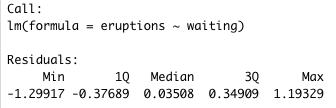
\includegraphics[scale=0.6]{images/regcall.png}
    \end{center}
    \begin{itemize}
        \item The first line shows the command used in \texttt{R} to run this regression model.
        \item The \texttt{Residuals} item shows a quartile-based summary of our residuals.
    \end{itemize}
\end{frame}

\begin{frame}{Regression Example}
    \begin{center}
        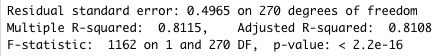
\includegraphics[scale=0.6]{images/regfstat.png}
    \end{center}
    The \texttt{F-statistic} and \texttt{p-value} give information about the model overall. 
    \begin{itemize}
        \item These are based on an F-distribution.
        \item The null hypothesis is that all of our model parameters are 0 (the model gives us no good info).
        \item Since p-value$ < 2.2\times10^{-16} < \alpha = 0.05$, at least one of the parameters is nonzero (the model is useful).
    \end{itemize}
\end{frame}

\begin{frame}{Regression Example}
    \begin{center}
        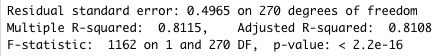
\includegraphics[scale=0.6]{images/regfstat.png}
    \end{center}
    \begin{itemize}
        \item \texttt{Multiple R-squared} is our squared correlation coefficient $R^2$. 
        \item This tells us how good our fit is.
        \item Ignore the adjusted R-squared and residual standard error for now.
    \end{itemize}
\end{frame}

\begin{frame}{Regression Example}
    \begin{center}
        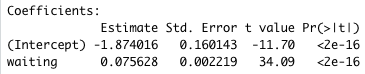
\includegraphics[scale=0.6]{images/regcoef.png}
    \end{center}
    Finally, the \texttt{Coefficients} section gives us several pieces of information:
    \begin{enumerate}
        \item \texttt{Estimate} shows the estimated parameters for each value.
        \item \texttt{Std. Error} gives the standard error for each parameter estimate.
        \item The \texttt{t values}s are the test statistics for each parameter estiamte.
        \item Finally, \texttt{Pr(>|t|)} are the p-values for each parameter estimate.
    \end{enumerate}
\end{frame}

\begin{frame}{Regression Example}
    The hypothesis test for each regression coefficient has hypotheses
    \begin{align*}
        H_0: \beta_i = 0 \\
        H_A: \beta_i \ne 0
    \end{align*}
    where $i=0$ for the intercept and $i=1$ for the slope.
\end{frame}

\begin{frame}{Regression Example}
    \begin{center}
        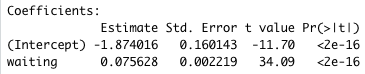
\includegraphics[scale=0.6]{images/regcoef.png}
    \end{center}
    \begin{itemize}
        \item $p-value < 2\times10^{-16}$ for $b_0$ so we can conclude that the intercept is nonzero.
        \item $p-value < 2\times10^{-16}$ for $b_1$ so we conclude that the intercept is also nonzero.
        \item This means that the intercept and slope both provide useful information when predicting values of $y=\texttt{eruptions}$.
    \end{itemize} 
\end{frame}

\begin{frame}{Confidence Intervals for a Coefficient}
    We can construct confidence intervals similar to those for hypothesis tests. A $(1-\alpha)100$\% confidence interval for $\beta_i$ is
    \[
        b_i \pm t_{\alpha/2}(df) \times SE(b_i)
    \]
    where the model df and SE can be found in the regression output.
\end{frame}

\begin{frame}{Aside: ANOVA for Regression Models}
    \begin{itemize}
        \item ANOVA will also play a role in regression.
        \item We can get the ANOVA table for a regression.
    \end{itemize}
\end{frame}

\begin{frame}{Aside: ANOVA for Regression Models}
    The ANOVA table in regression will look something like this: 
    \begin{table}[h]
        \centering
        \begin{tabular}{l cccccc}
             & Df & Sum Sq & Mean Sq & F value  &  Pr($>$F) \\
             \cline{2-6}
            faithful\$waiting & 1 & 286.478 & 286.478 & 1162.1 & $<$ 2.2e-16 \\
            Residuals & 270 & 66.562 & 0.247 & & \\ 
        \end{tabular}
    \end{table}
\end{frame}

\begin{frame}{Example}
    \begin{center}
        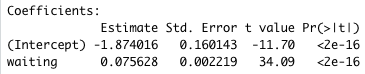
\includegraphics[scale=0.6]{images/regcoef.png}
    \end{center}
    Find 95\% confidence intervals for $\beta_0$ and $\beta_1$.
\end{frame}

\begin{frame}{Estimation and Prediction Using a Regression Line}
    We now know
    \begin{itemize}
        \item how to examine if a model is useful.
        \item how to confirm that our regression assumptions are satisfied.
    \end{itemize}
\end{frame}

\begin{frame}{Estimation and Prediction Using a Regression Line}
    Given a useful regression line, we want to 
    \begin{itemize}
        \item estimate an average value of $y$ for a given value of $x$.
        \item estimate a particular value of $y$ for a given value of $x$.
    \end{itemize}
\end{frame}

\begin{frame}{Estimation and Prediction Using a Regression Line}
    We've already talked about using a regression line to make predictions.
    \[
        \hat{y}=b_0 + b_1x
    \]
    Plug in $x$ and we get a good estimate for the \textit{average} value of $y$ at that point.
\end{frame}

\begin{frame}{Estimation and Prediction Using a Regression Line}
    Point estimates are useful, but we want to consider variability!
    \begin{itemize}
        \item Recall: one of our regression assumptions is normally distributed errors.
        \item This means that the variability around the regression line should be approximately normal 
        \begin{itemize}
            \item with mean $\beta_0 + \beta_1 x$
            \item and standard deviation $\sigma$.
        \end{itemize}
    \end{itemize}
\end{frame}

\begin{frame}{The Variability of $\hat{y}$}
    \begin{itemize}
        \item Notice that $\hat{y}$ is an estimator.
        \item The variability of an estimator is its standard error.
        \item Then $\sigma$ is well-approximated by 
    \end{itemize}
    \[
        SE(\hat{y}) = \sqrt{\text{MSE}\left(\frac{1}{n} + \frac{(x_0-\bar{x})^2}{s_x}\right)}
    \]
\end{frame}

\begin{frame}{The Variability of $\hat{y}$}
    Since we are working with a normal distribution, estimation and testing can be based on the test statistic
    \[
        t = \frac{\hat{y} - y_0}{SE(\hat{y})}
    \]
    which corresponds to a $t(n-2)$ distribution.
\end{frame}

\begin{frame}{Confidence Intervals for $y$}
    A $(1-\alpha)100$\% confidence interval for the average value of $y$ (measured by $\beta_0 + \beta_1 x$) when $x=x_0$ is
    \[
        \hat{y} \pm t_{\alpha/2}(n-2)\times SE(\hat{y}) 
    \]
    or
    \[
        \hat{y} \pm t_{\alpha/2}(n-2)\times 
        \sqrt{\text{MSE}\left(\frac{1}{n} + \frac{(x_0-\bar{x})^2}{s_x}\right)}
    \]
\end{frame}

\begin{frame}{Prediction Intervals for $y$}
    \begin{itemize}
        \item So far, we've only considered \textit{average} values of the outcome variable $y$.
        \item What if we wanted to predict a \textit{particular} value of $y$?
    \end{itemize}
\end{frame}

\begin{frame}{Prediction Intervals for $y$}
    For a residual,
    \[
        e = \epsilon + \text{error in estimating line}
    \]
    \begin{itemize}
        \item We don't know the true breakdown between these components.
        \item ...but we can use this concept to build a new standard error formula.
    \end{itemize}
\end{frame}

\begin{frame}{Prediction Intervals for $y$}
    The standard error of $(y-\hat{y})$ is
    \[
        SE(y-\hat{y}) = \sqrt{\text{MSE}\left(1 + \frac{1}{n} + \frac{(x_0-\bar{x})^2}{s_x}\right)}
    \]
\end{frame}

\begin{frame}{Prediction Intervals for $y$}
    A $(1-\alpha)100$\% \textbf{prediction interval} for a specific value of $y$ when $x=x_0$ is
    \[
        \hat{y} \pm t_{\alpha/2}(n-2)\times SE(y-\hat{y}) 
    \]
    or
    \[
        \hat{y} \pm t_{\alpha/2}(n-2)\times 
        \sqrt{\text{MSE}\left(1 + \frac{1}{n} + \frac{(x_0-\bar{x})^2}{s_x}\right)}
    \]
\end{frame}

\begin{frame}{Example}
    The regression line for the \texttt{faithful} data using \texttt{waiting} to predict \texttt{eruption} was
    \[
        \hat{y} = -1.874 + 0.076x
    \]
\end{frame}

\begin{frame}{Example}
    The ANOVA table for this regression is 
    \begin{table}[h]
        \centering
        \begin{tabular}{l cccccc}
             & Df & Sum Sq & Mean Sq & F value  &  Pr($>$F) \\
             \cline{2-6}
            faithful\$waiting & 1 & 286.478 & 286.478 & 1162.1 & $<$ 2.2e-16 \\
            Residuals & 270 & 66.562 & 0.247 & & \\ 
        \end{tabular}
    \end{table}
    \begin{enumerate}
        \item Find the appropriate interval for the average eruption time when the wait time is 70 minutes.
        \item Find the appropriate interval for the specific eruption time when the wait time is 70 minutes.
    \end{enumerate}
\end{frame}
